\documentclass[tikz,border=5pt]{standalone}
\usepackage{tikz}
\usetikzlibrary{arrows.meta, calc}
\usetikzlibrary{decorations.markings, arrows}
\usetikzlibrary{decorations.shapes}
\usetikzlibrary{decorations.pathreplacing}

% --- Define Colors ---
\definecolor{myblue}{RGB}{175, 204, 233}
\definecolor{mygreen}{RGB}{125,208,163}

\tikzstyle{blue} = [draw=none,outer sep=0, inner sep=5,
    minimum width=1cm, minimum height=1cm, 
    top color=myblue, bottom color=myblue, font=\Large, align=center]
\tikzstyle{green} = [draw=none,outer sep=0,inner sep=5,
    minimum width=1cm, minimum height=1cm, 
    top color=mygreen, bottom color=mygreen, font=\Large, align=center]


\tikzstyle{square} = [draw,outer sep=5,inner sep=3,minimum size=10,
    line width=0, very thick, draw=black!100,
    top color=white,bottom color=white, font=\Huge]


\begin{document}

% ==================================================================
% FIGURE : CONCURRENCY
% ==================================================================
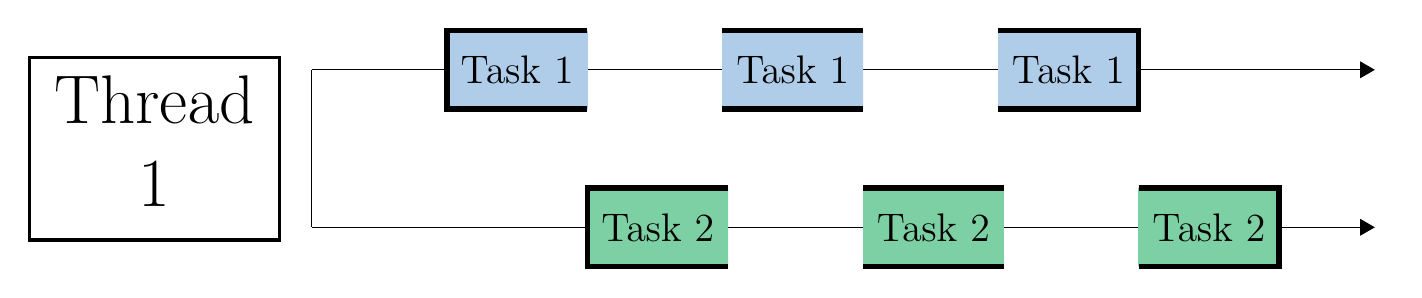
\begin{tikzpicture}

    % 1. Place the CPU
    \node[square] at (-3.5,0) {\begin{tabular}{c} Thread \\ 1 \end{tabular}};;


\draw[-triangle 60]  (-1.5,1) -- node[pos=1, anchor=west] {\textbf{\begin{tabular}{c} \end{tabular}}}(12,1);
\draw[-triangle 60]  (-1.5,-1) -- node[pos=1, anchor=west] {\textbf{\begin{tabular}{c} \end{tabular}}}(12,-1);
\draw (-1.5,1) -- (-1.5,-1);
%\draw[black,line width = 2, fill=myblue]  (t1.north west) -- (t1.north east) -- (t1.south east) -- (t1.south west);
%\node at (t1.center) {\Large Task 1};

%%% TASK 1
% Box with borders on top, left, bottom (no right)
\node[blue,anchor=east] (t2) at (2,1) {Task 1};
\draw[black,line width=2] (t2.north east) -- (t2.north west) -- (t2.south west) -- (t2.south east);

% Box with borders on top, right, bottom (no left)
\node[blue,anchor=east] (t1) at (5.5,1) {Task 1};
\draw[black,line width=2] (t1.north west) -- (t1.north east); % top
\draw[black,line width=2] (t1.south west) -- (t1.south east); % bottom

 
% Box with borders on top, left, bottom (no right)
\node[blue,anchor=east] (t3) at (9,1) {Task 1};
\draw[black,line width=2]  (t3.north west) -- (t3.north east) -- (t3.south east) -- (t3.south west);



%%% TASK 2
% Box with borders on top, left, bottom (no right)
\node[green, anchor=west] (s2) at (2,-1) {Task 2};
\draw[black,line width=2] (s2.north east) -- (s2.north west) -- (s2.south west) -- (s2.south east);

% Box with borders on top, right, bottom (no left)
\node[green, anchor=west] (s1) at (5.5,-1) {Task 2};
\draw[black,line width=2] (s1.north west) -- (s1.north east); % top
\draw[black,line width=2] (s1.south west) -- (s1.south east); % bottom

  
% Box with borders on top, left, bottom (no right)
\node[green,anchor=west] (s3) at (9,-1) {Task 2};
\draw[black,line width=2] (s3.north west) -- (s3.north east) -- (s3.south east) -- (s3.south west);



\end{tikzpicture}

\end{document}
